% Options for packages loaded elsewhere
\PassOptionsToPackage{unicode}{hyperref}
\PassOptionsToPackage{hyphens}{url}
%
\documentclass[
  english,
  man,floatsintext]{apa6}
\usepackage{lmodern}
\usepackage{amsmath}
\usepackage{ifxetex,ifluatex}
\ifnum 0\ifxetex 1\fi\ifluatex 1\fi=0 % if pdftex
  \usepackage[T1]{fontenc}
  \usepackage[utf8]{inputenc}
  \usepackage{textcomp} % provide euro and other symbols
  \usepackage{amssymb}
\else % if luatex or xetex
  \usepackage{unicode-math}
  \defaultfontfeatures{Scale=MatchLowercase}
  \defaultfontfeatures[\rmfamily]{Ligatures=TeX,Scale=1}
\fi
% Use upquote if available, for straight quotes in verbatim environments
\IfFileExists{upquote.sty}{\usepackage{upquote}}{}
\IfFileExists{microtype.sty}{% use microtype if available
  \usepackage[]{microtype}
  \UseMicrotypeSet[protrusion]{basicmath} % disable protrusion for tt fonts
}{}
\makeatletter
\@ifundefined{KOMAClassName}{% if non-KOMA class
  \IfFileExists{parskip.sty}{%
    \usepackage{parskip}
  }{% else
    \setlength{\parindent}{0pt}
    \setlength{\parskip}{6pt plus 2pt minus 1pt}}
}{% if KOMA class
  \KOMAoptions{parskip=half}}
\makeatother
\usepackage{xcolor}
\IfFileExists{xurl.sty}{\usepackage{xurl}}{} % add URL line breaks if available
\IfFileExists{bookmark.sty}{\usepackage{bookmark}}{\usepackage{hyperref}}
\hypersetup{
  pdftitle={Are we all on the same page? Subfield differences in open science practices in psychology},
  pdfauthor={Christina Riochios1 \& Jenny L. Richmond1},
  pdflang={en-EN},
  pdfkeywords={keywords},
  hidelinks,
  pdfcreator={LaTeX via pandoc}}
\urlstyle{same} % disable monospaced font for URLs
\usepackage{graphicx}
\makeatletter
\def\maxwidth{\ifdim\Gin@nat@width>\linewidth\linewidth\else\Gin@nat@width\fi}
\def\maxheight{\ifdim\Gin@nat@height>\textheight\textheight\else\Gin@nat@height\fi}
\makeatother
% Scale images if necessary, so that they will not overflow the page
% margins by default, and it is still possible to overwrite the defaults
% using explicit options in \includegraphics[width, height, ...]{}
\setkeys{Gin}{width=\maxwidth,height=\maxheight,keepaspectratio}
% Set default figure placement to htbp
\makeatletter
\def\fps@figure{htbp}
\makeatother
\setlength{\emergencystretch}{3em} % prevent overfull lines
\providecommand{\tightlist}{%
  \setlength{\itemsep}{0pt}\setlength{\parskip}{0pt}}
\setcounter{secnumdepth}{-\maxdimen} % remove section numbering
% Make \paragraph and \subparagraph free-standing
\ifx\paragraph\undefined\else
  \let\oldparagraph\paragraph
  \renewcommand{\paragraph}[1]{\oldparagraph{#1}\mbox{}}
\fi
\ifx\subparagraph\undefined\else
  \let\oldsubparagraph\subparagraph
  \renewcommand{\subparagraph}[1]{\oldsubparagraph{#1}\mbox{}}
\fi
% Manuscript styling
\usepackage{upgreek}
\captionsetup{font=singlespacing,justification=justified}

% Table formatting
\usepackage{longtable}
\usepackage{lscape}
% \usepackage[counterclockwise]{rotating}   % Landscape page setup for large tables
\usepackage{multirow}		% Table styling
\usepackage{tabularx}		% Control Column width
\usepackage[flushleft]{threeparttable}	% Allows for three part tables with a specified notes section
\usepackage{threeparttablex}            % Lets threeparttable work with longtable

% Create new environments so endfloat can handle them
% \newenvironment{ltable}
%   {\begin{landscape}\centering\begin{threeparttable}}
%   {\end{threeparttable}\end{landscape}}
\newenvironment{lltable}{\begin{landscape}\centering\begin{ThreePartTable}}{\end{ThreePartTable}\end{landscape}}

% Enables adjusting longtable caption width to table width
% Solution found at http://golatex.de/longtable-mit-caption-so-breit-wie-die-tabelle-t15767.html
\makeatletter
\newcommand\LastLTentrywidth{1em}
\newlength\longtablewidth
\setlength{\longtablewidth}{1in}
\newcommand{\getlongtablewidth}{\begingroup \ifcsname LT@\roman{LT@tables}\endcsname \global\longtablewidth=0pt \renewcommand{\LT@entry}[2]{\global\advance\longtablewidth by ##2\relax\gdef\LastLTentrywidth{##2}}\@nameuse{LT@\roman{LT@tables}} \fi \endgroup}

% \setlength{\parindent}{0.5in}
% \setlength{\parskip}{0pt plus 0pt minus 0pt}

% \usepackage{etoolbox}
\makeatletter
\patchcmd{\HyOrg@maketitle}
  {\section{\normalfont\normalsize\abstractname}}
  {\section*{\normalfont\normalsize\abstractname}}
  {}{\typeout{Failed to patch abstract.}}
\patchcmd{\HyOrg@maketitle}
  {\section{\protect\normalfont{\@title}}}
  {\section*{\protect\normalfont{\@title}}}
  {}{\typeout{Failed to patch title.}}
\makeatother
\shorttitle{Subfield differences in open science practices}
\keywords{keywords\newline\indent Word count: X}
\usepackage{lineno}

\linenumbers
\usepackage{csquotes}
\usepackage[titles]{tocloft}
\cftpagenumbersoff{figure}
\renewcommand{\cftfigpresnum}{\itshape\figurename\enspace}
\renewcommand{\cftfigaftersnum}{.\space}
\setlength{\cftfigindent}{0pt}
\setlength{\cftafterloftitleskip}{0pt}
\settowidth{\cftfignumwidth}{Figure 10.\qquad}
\ifxetex
  % Load polyglossia as late as possible: uses bidi with RTL langages (e.g. Hebrew, Arabic)
  \usepackage{polyglossia}
  \setmainlanguage[]{english}
\else
  \usepackage[shorthands=off,main=english]{babel}
\fi
\ifluatex
  \usepackage{selnolig}  % disable illegal ligatures
\fi
\newlength{\cslhangindent}
\setlength{\cslhangindent}{1.5em}
\newlength{\csllabelwidth}
\setlength{\csllabelwidth}{3em}
\newenvironment{CSLReferences}[2] % #1 hanging-ident, #2 entry spacing
 {% don't indent paragraphs
  \setlength{\parindent}{0pt}
  % turn on hanging indent if param 1 is 1
  \ifodd #1 \everypar{\setlength{\hangindent}{\cslhangindent}}\ignorespaces\fi
  % set entry spacing
  \ifnum #2 > 0
  \setlength{\parskip}{#2\baselineskip}
  \fi
 }%
 {}
\usepackage{calc}
\newcommand{\CSLBlock}[1]{#1\hfill\break}
\newcommand{\CSLLeftMargin}[1]{\parbox[t]{\csllabelwidth}{#1}}
\newcommand{\CSLRightInline}[1]{\parbox[t]{\linewidth - \csllabelwidth}{#1}\break}
\newcommand{\CSLIndent}[1]{\hspace{\cslhangindent}#1}

\title{Are we all on the same page? Subfield differences in open science practices in psychology}
\author{Christina Riochios\textsuperscript{1} \& Jenny L. Richmond\textsuperscript{1}}
\date{}


\authornote{

School of Psychology, UNSW

The authors made the following contributions. Christina Riochios: Conceptualization, Methodology, Investigation, Data curation, Visualisation, Formal Analysis, Writing - Original Draft Preparation, Writing - Review \& Editing; Jenny L. Richmond: Conceptualization, Methodology, Formal Analysis, Writing - Original Draft Preparation, Writing - Review \& Editing, Supervision.

}

\affiliation{\vspace{0.5cm}\textsuperscript{1} University of New South Wales}

\abstract{
Although open science has become a popular tool to combat the replication crisis, it is unclear whether the uptake of open science practices has been consistent across the field of psychology. In this study, we utilised open data from a previous study to determine whether data and material sharing, two prominent open science practices, differed as a function of psychological subfield at the distinguished journal, \emph{Psychological Science}. The results showed that open data and open materials scores, indicators of data and material sharing, increased from 2014-2015 to 2019-2020. Of note, articles published in the field of developmental psychology generated considerably lower open data and open materials scores, compared to articles in other subfields. These findings are discussed in the context of why developmental psychologists may be slower to adopt open science practices, compared to other researchers, and how journals can more effectively encourage authors to practice open science, across all psychological subfields. As part of our analyses, we also looked at how the awarding of Open Science Badges related to researchers' open science behaviours. Whilst Open Science Badges were closely related to data and material sharing, the shared data and materials were less usable expected. We propose an alternative open science initiative, that may be more effective in increasing the replicability of psychological research.
}



\begin{document}
\maketitle

The field of psychology, like many other scientific disciplines, is currently facing a replication crisis, in which researchers are struggling to replicate existing findings. In 2015, a group of 270 psychological researchers attempted to replicate the findings of 100 psychology experiments. Whilst 97\% of the original studies generated statistically significant findings, only 36\% of the replication attempts were statistically significant. In addition, the replicated effects were, on average, half the size of the original effects (Open Science Collaboration, 2015). These findings illustrate the poor replicability of psychological research and the pressing need to rectify flawed research practices.

Open science practices, which increase the transparency of, and access to, scientific research, have been used to combat the replication crisis within psychology. (Klein et al., 2018). Open data and open materials practices, for example, involve researchers sharing their raw data and experimental materials on publicly accessible online repositories. These practices make it easier for others to replicate the methodology and reproduce the results from published work (Klein et al., 2018).

To encourage researchers to employ open science practices, many psychology journals have implemented incentives, like Open Science Badges. In 2013, the Center for Open Science established three Open Science Badges (Open Data, Open Materials and Preregistered) to acknowledge and reward researchers for their use of open science practices (Center for Open Science, 2021). The Open Data and Open Materials Badges, for example, are awarded when the data and materials that are required to reproduce the methods and results of a study are shared publicly online. To date, over 75 journals (40 in Psychology) have adopted Open Science Badges (Center for Open Science, 2021).

At \emph{Psychological Science}, the Association of Psychological Science's flagship journal, Open Science Badges appear to have been successful in encouraging researchers to adopt open science practices. In 2016, Kidwell et al.~coded the frequency of data and material sharing in the 18 months before and after Open Science Badges were implemented at \emph{Psychological Science}. Kidwell et al.~found that data sharing increased dramatically from 2.5\% of articles prior to badges to 39.4\% of articles following badges. Materials sharing also rose from 12.7\% to 30.3\%. Data and material sharing in control journals, such as the \emph{Journal of Personality and Social Psychology}, which did not award badges, remained low over the same time period (Kidwell et al., 2016). Although their results simply described the proportion of articles that engaged in data and materials sharing before and after the policy change, the results led Kidwell et al.~to conclude that Open Science Badges successfully incentivised the uptake of open science practices at \emph{Psychological Science}.

The support for open science continues to grow, however, it is not yet clear whether engagement with open science is consistent across different fields within psychology. Notably, the field of developmental psychology has received significant criticism for its lack of receptivity towards open science. As Figure 1 illustrates, prominent developmental researchers, Prof Michael Frank and Dr.~Jennifer Pfeifer, have labelled the Society for Research in Child Development's (SRCD) open science policy as `weak' and as one that `undervalues openness.'(Frank, 2020, March 6; Pfeifer, 2020, March 8). More recently, the Editor-in-Chief of Infant and Child Development, Prof Moin Syed, stated that the uptake of open science within the field of developmental psychology has been `slow and uneven' (Syed, 2021). A survey supporting these viewpoints showed that 80\% of researchers publishing in \emph{Child Development} felt their institutions failed to provide adequate guidance or financial support for sharing data (SRCD Task Force on Scientific Integrity and Openness Survey (2017), cited in Gennetian et al., (2020)). Developmental psychology researchers may be slower to adopt open science practices than those in other psychological disciplines, however, this possibility has yet to be empirically investigated.

\begin{figure}

{\centering 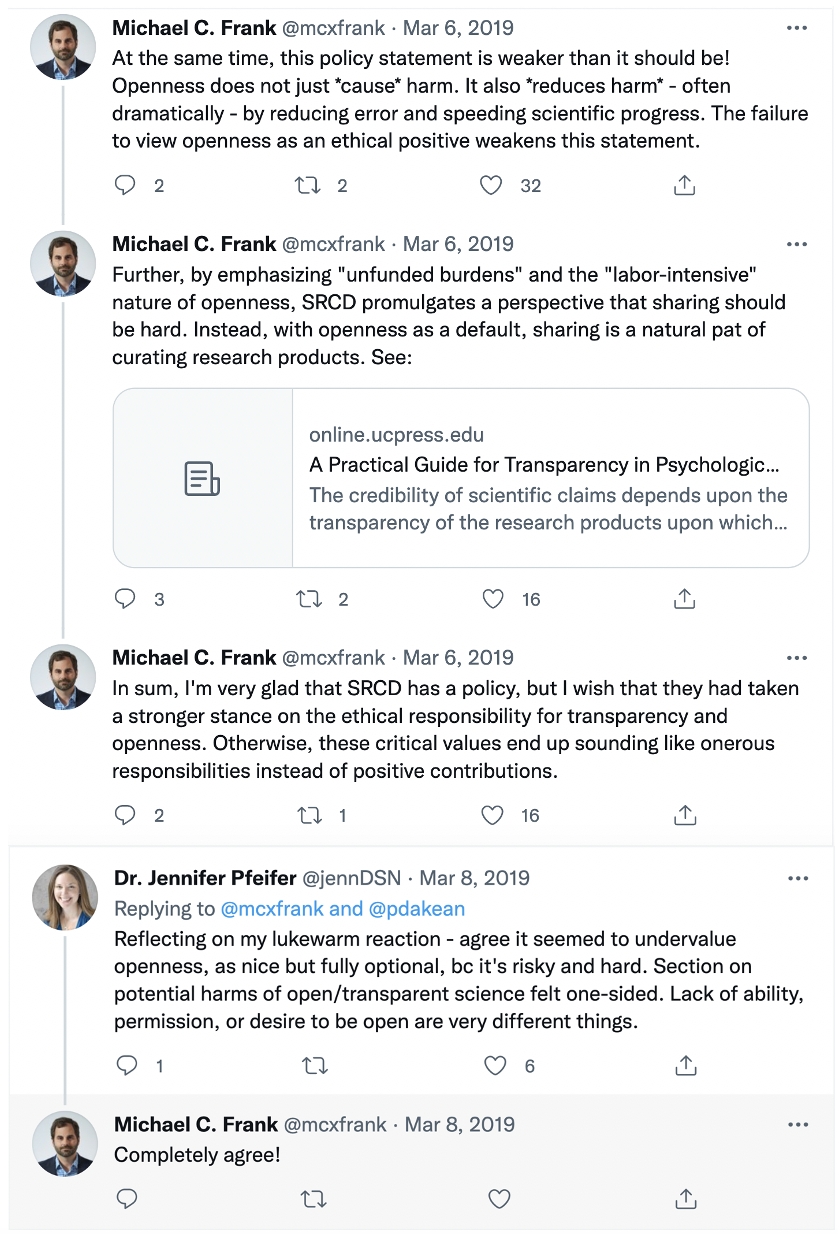
\includegraphics[width=2.79in]{/Users/jenny/Desktop/Desktop - N591/git/same_page/Manuscript/Figure 1} 

}

\caption{Twitter thread about Society for Child Development open science policy.}\label{fig:unnamed-chunk-1}
\end{figure}

Using meta-research, the study of research itself, we can empirically assess whether developmental psychology is truly behind in the open science movement. Previous investigations, including Kidwell et al. (2016), have revealed that open science incentives can increase the use of open science practices. However, it is unclear whether Open Science Badges, have had the same impact across different psychological subfields and whether the effect is sustained over time. To address this research question, we used the open data from the Kidwell et al., (2016) study and designed a quantitative scoring system to examine whether rates of data and material sharing, following the implementation of Open Science Badges at \emph{Psychological Science}, differed as a function of subfield. In addition, we applied the same scoring system to articles published in the most recent 18 months (Jul 2019-Dec 2020) to test whether the badges have continued to be impactful and whether the impact has been consistent across subfields. We were particularly interested in determining whether developmental psychology researchers publishing in \emph{Psychological Science} engaged with open science practices at the same rate as researchers from other subdomains of psychology. Our methods and analysis plan were preregistered at the Open Science Framework: \url{https://osf.io/3tsmy/}.

\hypertarget{methods}{%
\section{Methods}\label{methods}}

\hypertarget{design}{%
\subsection{Design}\label{design}}

This study had a quasi-experimental design; all articles were systematically assigned to one of seven subfields. For each article, we used coded variables to compute two scores that indexed the transparency of data and materials, respectively. Changes in data and material sharing were analysed over six-month intervals.

\hypertarget{sample}{%
\subsection{Sample}\label{sample}}

The Kidwell et al., (2016) sample comprised of all \emph{Psychological Science} articles published between January 2014 and May 2015 (N = 367), which were coded to evaluate the openness of their data and materials. To identify how data and material sharing may have changed since 2014-2015, our sample also included all \emph{Psychological Science} articles that were published between July 2019 and December 2020 (N = 242). Non-empirical articles that did not contain an experiment or analysis, including editorials, commentaries, replies, corrigenda, errata and retractions, were excluded from our analysis. After filtering out these non-empirical articles from the sample, 322 articles published between 2014-2015 and 193 articles published between 2019-2020, remained.

\hypertarget{materials}{%
\subsection{Materials}\label{materials}}

To assess the transparency of data and materials for each article, Kidwell et al.~(2016) employed a systematic coding system (\url{https://osf.io/j4x23/}; variable definitions \url{https://osf.io/j4x23/}). We downloaded the data Kidwell et al.~coded from their OSF repository (\url{https://osf.io/rfgdw/}) and filtered the dataset to only include data from \emph{Psychological Science} articles published between January 2014 and May 2015.
In addition to the variables that Kidwell et al.~had coded, we also coded for whether the article specified their analysis software or not, and which type of analysis software had been specified (e.g., R, JASP, SPSS etc). These variables were important to include because when authors' identify their analysis software, the analysis procedure can be easier to follow and the chance of successfully reproducing the analysis may increase (National Academies of Sciences, Medicine, \& others, 2019).
The same amended version of the Kidwell et al.~coding system, including the two additional analysis software variables, was used to code the articles that were published between July 2019 and December 2020.

We designed an additional coding system (\url{https://osf.io/a9vgr/}; variable definitions \url{https://osf.io/md5eu/}) to assign all the articles to one of seven psychological subfields: Developmental Psychology, Social Psychology, Cognition, Perception, Health Psychology, Cognitive Neuroscience and Behavioural Neuroscience. We identified these seven subfields as those that the vast majority of \emph{Psychological Science} articles fall into, after thoroughly reviewing the journal website.

Prior to data collection, each member of the coding team coded five trial articles, to confirm their understanding of the coding process. These trial articles were \emph{Psychological Science} articles originally coded by Mallory Kidwell, the primary investigator in the Kidwell et al.~(2016) study. Kidwell's coding acted as the standard to which coders' responses were compared. The senior coder in the current study generated the standard for the variables that weren't included in the Kidwell et al.~coding system. The trial articles varied in the transparency of their data and materials, and therefore, exposed coders to a representative range of coding outcomes.

The coding team coded both the trial and target articles via a Qualtrics survey, containing a series of multiple-choice questions. The questions were structured in an `if-then' manner, with some questions only being asked if coders provided particular answers to the questions prior. For example, coders were only asked about the participants' age, if they had specified that the participants in the study were `Humans' as opposed to `Animals.'

\hypertarget{procedure}{%
\subsection{Procedure}\label{procedure}}

After the investigation had been approved by the Human Research Ethics Advisory Panel, we assembled a team of volunteer coders, comprising of undergraduate UNSW psychology students. Once the coders coded the five trial articles and the senior coder was confident that each coder understood how to code all the variables correctly, the coders were provided access to the target set of articles to begin coding using the Qualtric survey.

\hypertarget{scoring-procedure}{%
\subsubsection{Scoring procedure}\label{scoring-procedure}}

After all articles had been coded, we imported the data from Qualtrics into the software environment, R (R Core Team, 2020). For the articles that were published between 2014-2015, we combined the newly collected data with the relevant Kidwell et al.~(2016) data. Each article, across both the 2014-2015 and 2019-2020 datasets, was assigned to one of the seven psychological subfields, and received an open data and open materials score. The open data score indexed the extent to which its data were transparent, whilst the open materials score indexed the extent to which the materials were transparent. Therefore, to calculate the scores, we weighted each coded variable according to how much it improved the transparency of the data and materials, respectively.

\emph{Table 1}: Open data scoring (left) and open materials scoring (right) criteria

\begin{figure}

{\centering 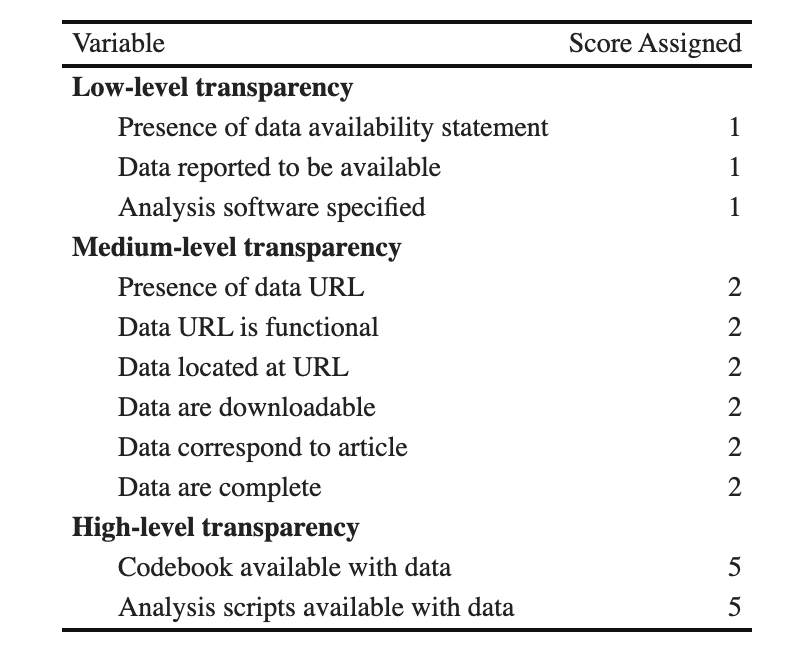
\includegraphics[width=0.49\linewidth,height=0.2\textheight]{data_scoring} 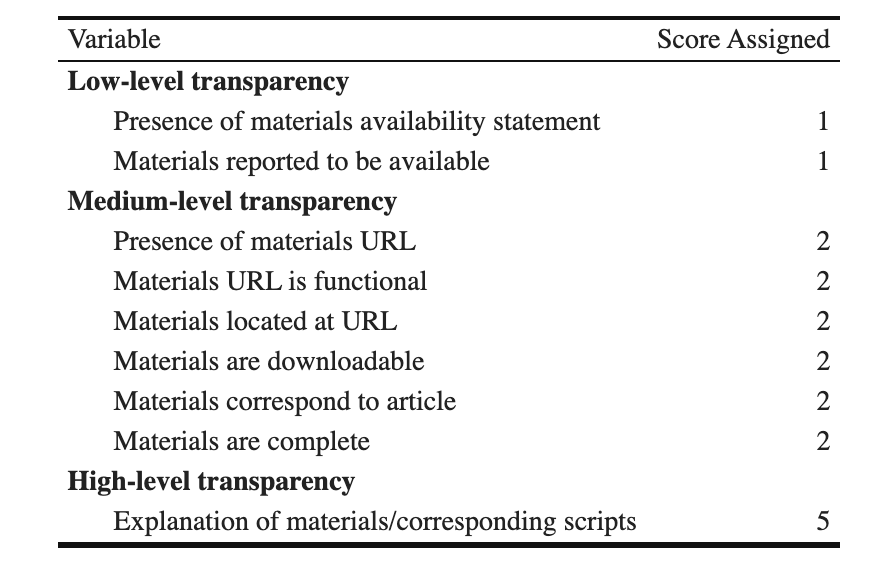
\includegraphics[width=0.49\linewidth,height=0.2\textheight]{mat_scoring} 

}

\end{figure}

There were three levels of transparency: low-level transparency variables received a value of 1, moderate-level transparency variables received a value of 2 and high-level transparency variables received a value of 5 (see Table 1 \& 2). We summed these scores so that each article received an open data score out of a possible 25 and an open materials score out of a possible 19. Higher scores reflected a higher level of transparency.

\hypertarget{reliability}{%
\subsubsection{Reliability}\label{reliability}}

After the 2014-2015 sample of articles had been coded, the senior coder randomly selected 25 empirical articles from the dataset (8\% of the empirical sample), ensuring that an equal number had been coded by each coder (n = 5), and double-coded these articles. Using the `kappa2' function from the `irr' package in R (Gamer, Lemon, \& Singh, 2019), we ran a Cohen's Kappa reliability analysis for subfield assignment, which revealed that the coding team had good reliability compared to the senior coder's standard, k = .605, according to Fleiss's (1981) guidelines. The percent agreement rating between the standard and the coding team was 72\%. Upon examining cases where the standard and the coding team disagreed on an article's subfield assignment, we found that the discrepancy could usually be attributed to the subject matter spanning across multiple subfields. Since our coding system did not account for the possibility of a study belonging to multiple subfields, the results from our reliability analysis may be conservative.

For the 2019-2020 sample of articles, the senior coder similarly selected 25 articles from the empirical sample (13\%) and double-coded these articles. Each article received a total openness score, representing the sum of the open data and open materials score. To assess reliability, we used the `icc' function from the `irr' package in R to generate an intraclass correlation coefficient (ICC) (Gamer, Lemon, \& Singh, 2019). The `tolerance' level was set at five Total Openness points; where scores fell within a five-point range of each other, they were considered to be equivalent.
The ICC analysis showed that the coding team had excellent reliability relative to the senior coder's standard, according to Cicchetti's (1994) guidelines, ICC = .905, 95\% CI (.772, .962). As a secondary measure of inter-rater reliability, we also calculated the percent agreement between the standard and coders' responses, for both the 2014-2015 and 2019-2020 datasets. The agreement rating between the coders and the standard was 73.7\%, with a tolerance level of five Total Openness points.

\hypertarget{data-analysis}{%
\subsubsection{Data analysis}\label{data-analysis}}

We used R {[}Version 4.0.3; R Core Team (2020){]} and the R-packages \emph{afex} {[}Version 1.0.1; Singmann, Bolker, Westfall, Aust, and Ben-Shachar (2021){]}, \emph{apa} {[}Version 0.3.3; Gromer (2020); Aust and Barth (2020){]}, \emph{dplyr} {[}Version 1.0.7; Wickham, François, Henry, and Müller (2021){]}, \emph{forcats} {[}Version 0.5.1; Wickham (2021a){]}, \emph{ggeasy} {[}Version 0.1.3; Carroll, Schep, and Sidi (2021){]}, \emph{gghalves} {[}Version 0.1.1; Tiedemann (2020){]}, \emph{ggplot2} {[}Version 3.3.5; Wickham (2016){]}, \emph{ggsignif} {[}Version 0.6.3; Constantin and Patil (2021){]}, \emph{goodshirt} {[}Version 0.2.2; Gruer (2021){]}, \emph{here} {[}Version 1.0.1; Müller (2020){]}, \emph{irr} {[}Version 0.84.1; Gamer, Lemon, and Singh (2019){]}, \emph{janitor} {[}Version 2.1.0; Firke (2021){]}, \emph{kableExtra} {[}Version 1.3.4; Zhu (2021){]}, \emph{lme4} {[}Version 1.1.27.1; Bates, Mächler, Bolker, and Walker (2015){]}, \emph{Matrix} {[}Version 1.3.4; Bates and Maechler (2021){]}, \emph{papaja} {[}Version 0.1.0.9997; Aust and Barth (2020){]}, \emph{patchwork} {[}Version 1.1.1; Pedersen (2020){]}, \emph{purrr} {[}Version 0.3.4; Henry and Wickham (2020){]}, \emph{readr} {[}Version 2.0.1; Wickham and Hester (2021){]}, \emph{report} {[}Version 0.3.5; Makowski, Ben-Shachar, Patil, and Lüdecke (2021){]}, \emph{scales} {[}Version 1.1.1; Wickham and Seidel (2020){]}, \emph{stringr} {[}Version 1.4.0; Wickham (2019){]}, \emph{tibble} {[}Version 3.1.4; Müller and Wickham (2021){]}, \emph{tidyr} {[}Version 1.1.3; Wickham (2021b){]}, and \emph{tidyverse} {[}Version 1.3.1; Wickham et al. (2019){]} for all our analyses.

\textbf{Confirmatory Analyses.} Analysis of Variance (ANOVA) analyses were run to investigate differences in open data and open materials scores, separately, across the 2014-2015 and 2019-2020 datasets. In each analysis, we tested for a main effect of time, measured over three six-month intervals, and subfield. To ensure that there was a comparable number of articles in each subfield group, we combined Cognitive Neuroscience, Behavioural Neuroscience, Health Psychology and Perception into a single `Other' category. As a result, a total of four subfield groups were included in our analysis: Developmental Psychology, Social Psychology, Cognition and Other. We report effect sizes in terms of generalised eta squared (ges).

\textbf{Exploratory Analyses.} After data collection, we were also interested in the distribution of scores and how the spread of scores might differ by subfield. To illustrate this we generated two raincloud plots that illustrated the distribution of open data and open materials scores across 2019-2020. Raincloud plots visualise the distribution of scores in a dataset by showing the density of subjects at each level of the dependent measure (Allen, Poggiali, Whitaker, Marshall, \& Kievit, 2019). In our case, where the violin plot was wider, the concentration of articles that received the corresponding open data or open materials score, was greater.

We also wanted to learn how Open Science Badges related to researchers' data and materials sharing practices. To generate two corresponding figures, we filtered the 2019-2020 dataset to only include the articles that had received an Open Data Badge and an Open Materials Badge, respectively. We then plotted the percentage of these articles that met a series of data and materials sharing criteria, described in the Results section below.

\hypertarget{preregistration}{%
\subsubsection{Preregistration}\label{preregistration}}

We preregistered our aims, hypotheses, design, and planned analysis procedure for the study at the OSF: \url{https://osf.io/3tsmy/}. Whilst we attempted to follow each of the proposed procedures as closely as possible, we made one notable modification. Namely, we chose not to normalise the Open Data and Open Materials Scores (so that they were both out of 100). Since our study was focussed on measuring subfield differences and changes over time, within each type of score, rather than comparing the differences between the two scores, we ultimately realised that normalising the scores was not necessary. All the materials, data and analysis scripts from the study can be accessed via the OSF: \url{https://osf.io/z8b7j/}.

\hypertarget{results}{%
\section{Results}\label{results}}

We first used the open data from Kidwell et al., (2016) and analysed whether open data and open materials scores improved across the 2014-2015 period and differed by subfield. As illustrated in Figure 2A, for open data scores the main effect of subfield, \(F(3, 310) = 2.23\), \(\mathit{MSE} = 41.51\), \(p = .085\), \(\hat{\eta}^2_G = .021\), was not significant, indicating that during the period immediately following the badge policy change, open data scores were uniformly low across subfields. Whilst open data scores increased over time,\(F(2, 310) = 11.29\), \(\mathit{MSE} = 41.51\), \(p < .001\), \(\hat{\eta}^2_G = .068\), this improvement did not differ as a function of subfield \(F(6, 310) = 1.57\), \(\mathit{MSE} = 41.51\), \(p = .157\), \(\hat{\eta}^2_G = .029\).

\begin{figure}
\centering
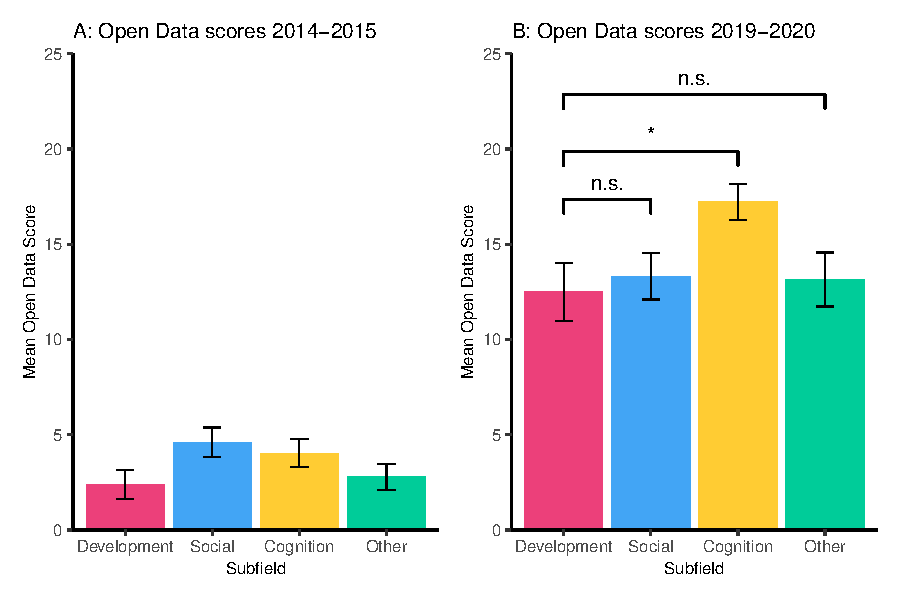
\includegraphics{icd_special_issue_files/figure-latex/unnamed-chunk-3-1.pdf}
\caption{\label{fig:unnamed-chunk-3}Mean open data scores for articles published in \emph{Psychological Science} between 2014-2015 and 2019-2020 as a function of subfield.}
\end{figure}

Across the 2019-2020 period, open data scores also increased significantly, \(F(2, 181) = 3.68\), \(\mathit{MSE} = 70.92\), \(p = .027\), \(\hat{\eta}^2_G = .039\), and differed by subfield, \(F(3, 181) = 3.31\), \(\mathit{MSE} = 70.92\), \(p = .021\), \(\hat{\eta}^2_G = .052\). When we compared the open data scores from papers published in developmental psychology to each of the other subfield categories (Figure 2B), we found that papers in developmental psychology had significantly lower open data scores (\emph{M} = 12.50, \emph{SD} = 8.83) than papers in cognition (\emph{M} = 17.23, \emph{SD} = 7.37), \(t(58.75) = -2.65\), \(p = .010\), but did not differ from papers published in social psychology (\emph{M} = 13.32, \emph{SD} = 9.17), \(t(71.68) = -0.42\), \(p = .675\) or those that fell into the other category (\emph{M} = 13.15, \emph{SD} = 9.07), \(t(71.12) = -0.31\), \(p = .756\). There was no significant time by subfield interaction, \(F(6, 181) = 1.11\), \(\mathit{MSE} = 70.92\), \(p = .358\), \(\hat{\eta}^2_G = .035\).

\begin{figure}
\centering
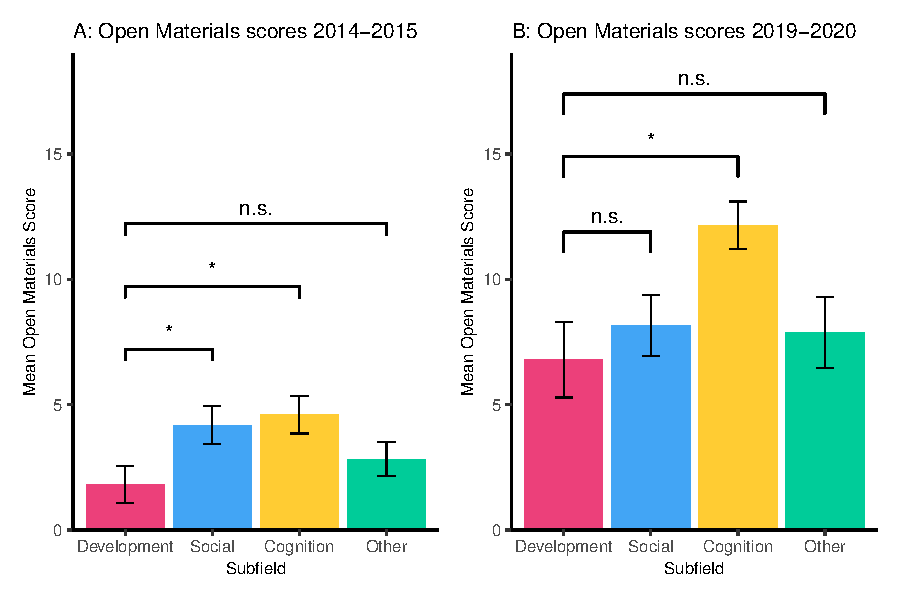
\includegraphics{icd_special_issue_files/figure-latex/unnamed-chunk-4-1.pdf}
\caption{\label{fig:unnamed-chunk-4}Mean open materials scores for articles published in \emph{Psychological Science} between 2014-2015 and 2019-2020 as a function of subfield.}
\end{figure}

For open materials scores across 2014-2015, there were significant main effects of both subfield, \(F(3, 310) = 4.03\), \(\mathit{MSE} = 32.16\), \(p = .008\), \(\hat{\eta}^2_G = .038\), and time period, \(F(2, 310) = 4.74\), \(\mathit{MSE} = 32.16\), \(p = .009\), \(\hat{\eta}^2_G = .030\) (see Figure 3A). Papers in developmental psychology had lower open materials scores (\emph{M} = 1.82, \emph{SD} = 6.02) than those in both social (\emph{M} = 4.19, \emph{SD} = 7.34), \(t(153.62) = -2.75\), \(p = .007\), and cognition (\emph{M} = 4.59, \emph{SD} = 7.07), \(t(153.74) = -3.20\), \(p = .002\), but developmental open materials scores did not differ from papers allocated to the other subfield category (\emph{M} = 2.83, \emph{SD} = 5.84), \(t(137.95) = -1.19\), \(p = .236\). The interaction between time period and subfield, \(F(6, 310) = 0.85\), \(\mathit{MSE} = 32.16\), \(p = .530\), \(\hat{\eta}^2_G = .016\), was not statistically significant.

As illustrated in Figure 3B, there were also subfield differences in open materials scores during the 2019-2020 period, \(F(3, 181) = 5.24\), \(\mathit{MSE} = 53.87\), \(p = .002\), \(\hat{\eta}^2_G = .080\). Consistent with open data scores, papers published in developmental psychology had significantly lower open materials scores (\emph{M} = 6.79, \emph{SD} = 8.83) than papers published in cognition, (\emph{M} = 6.79, \emph{SD} = 8.83), \(t(61.36) = -3.45\), \(p = .001\), however, open materials scores did not differ between developmental and social psychology (\emph{M} = 6.79, \emph{SD} = 8.83), \(t(68.36) = -0.84\), \(p = .406\), nor between developmental psychology and the other subfield category (\emph{M} = 6.79, \emph{SD} = 8.83), \(t(70.45) = -0.62\), \(p = .539\). There were no changes in open materials scores across the time period between mid-2019 and the end of 2020, \(F(2, 181) = 0.37\), \(\mathit{MSE} = 53.87\), \(p = .694\), \(\hat{\eta}^2_G = .004\), and differences in subfield did not vary over time, \(F(6, 181) = 0.48\), \(\mathit{MSE} = 53.87\), \(p = .822\), \(\hat{\eta}^2_G = .016\).

\begin{figure}
\centering
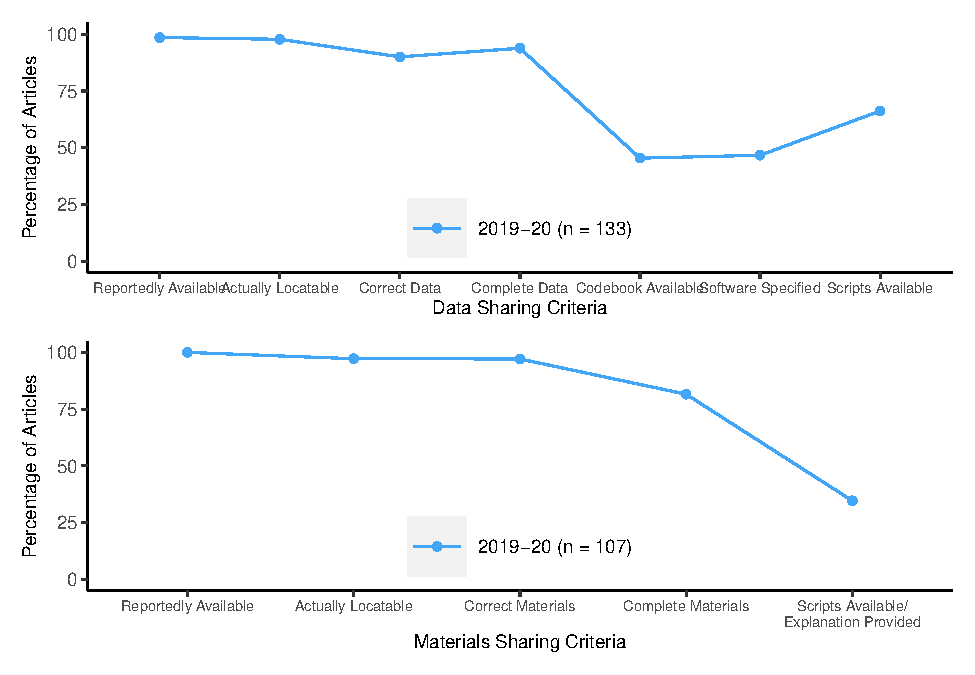
\includegraphics{icd_special_issue_files/figure-latex/unnamed-chunk-5-1.pdf}
\caption{\label{fig:unnamed-chunk-5}Mean open data and open materials scores for articles published in \emph{Psychological Science} as a function of subfield and time period.}
\end{figure}

It is clear that since the introduction of Open Science Badges in 2014, papers published in \emph{Psychological Science} have become more open over time and that most recently, developmental psychology has lagged behind some, but not all, subfields. To determine whether the rate of improvement from 2014-2015 through 2019-2020 differed significantly by subfield, we combined the data across the two coded time periods and looked for subfield by time interactions in both open data and open materials scores. As illustrated in Figure 4, there was no evidence that the magnitude of improvement over time differed by subfield for either both open data scores \(F(3, 507) = 2.28\), \(\mathit{MSE} = 55.28\), \(p = .078\), \(\hat{\eta}^2_G = .013\) or open materials scores \(F(3, 507) = 2.07\), \(\mathit{MSE} = 40.21\), \(p = .103\), \(\hat{\eta}^2_G = .012\).

\begin{figure}
\centering
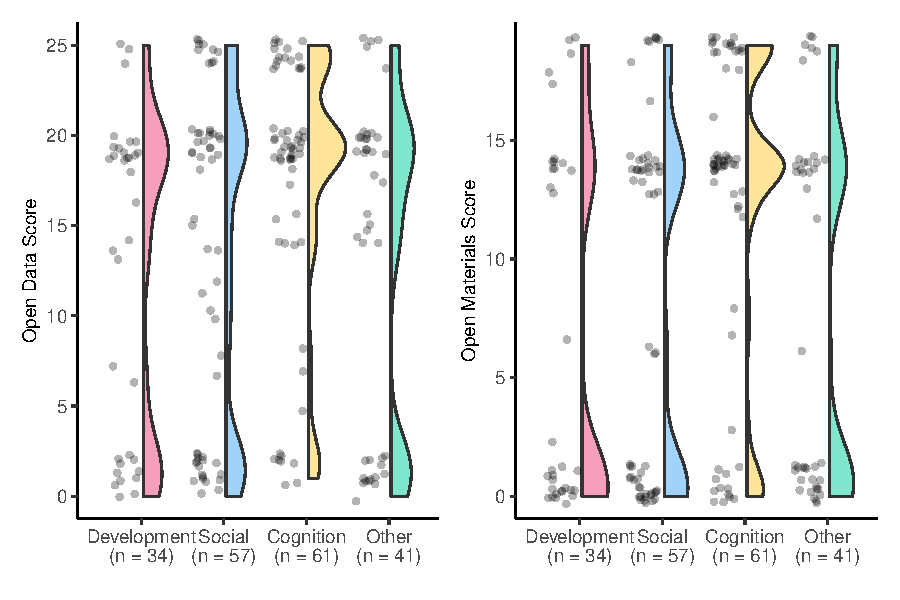
\includegraphics{icd_special_issue_files/figure-latex/rain-1.pdf}
\caption{\label{fig:rain}Distribution of open data and open materials scores earned by articles published in \emph{Psychological Science} between 2019 and 2020 as a function of subfield}
\end{figure}

Our confirmatory analyses showed that on average, open data and materials scores for papers published in \emph{Psychological Science} have increased markedly across all subfields, however, scores within each subfield varied widely. To capture changes in variability over time, we used raincloud plots (Allen, Poggiali, Whitaker, Marshall, \& Kievit, 2019) to represent the distribution of open data and materials scores across subfields. Figure 5 illustrates that in 2014-2015, across all subfields, most open data and open materials scores were low, with between 70-80\% of papers receiving scores less than 5. In contrast in 2019-2020, the majority of papers score on the upper half of the scale, however, there are still one third of papers published that receive scores less than 5.

\begin{figure}
\centering
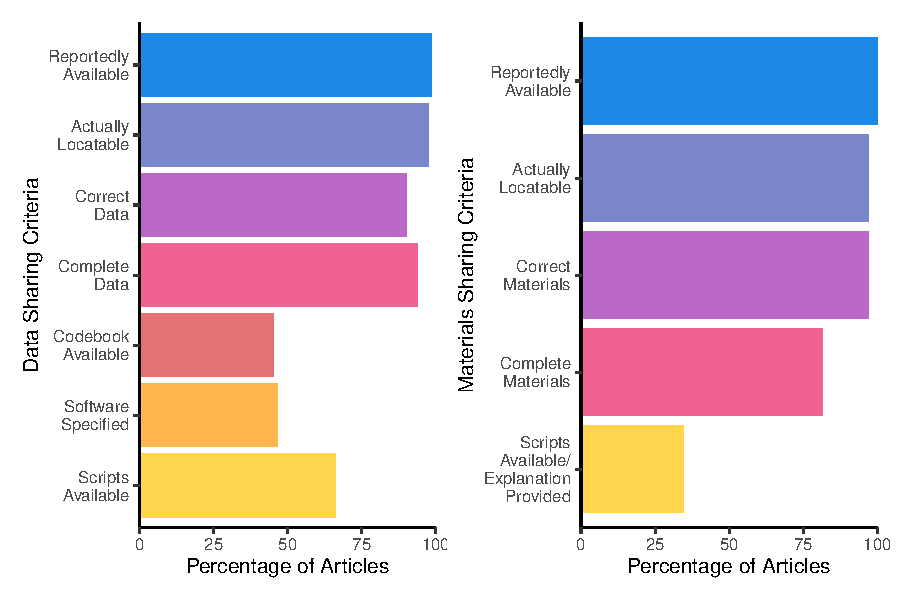
\includegraphics{icd_special_issue_files/figure-latex/unnamed-chunk-6-1.pdf}
\caption{\label{fig:unnamed-chunk-6}Proportion of articles published in \emph{Psychological Science} in 2019-2020 that earned an Open Data Badge (left) or Open Materials Badge (right) and engaged with sharing criteria behaviours}
\end{figure}

We were surprised how few articles received very high open data and materials scores even in 2019-2020. In order to receive very high scores, article authors needed to engage in behaviours that make shared resources most useful (i.e.~sharing data with a accompanying codebook and analysis script). We were particularly interested in how common this kind of metadata sharing was among papers that had earned an Open Data or Open Materials Badge. To produce Figure 6, we filtered articles published within the 2019-2020 window for those that were awarded open data and materials badges and then plotted the proportion of those articles that shared codebooks and scripts along with complete data.

The vast majority of papers earning an open data badge had complete data available, less than half shared a codebook and only 66\% included a analysis script. Similarly for open materials, most articles earning a badge shared raw materials on an open repository but a relatively small percentage of articles also shared an script and/or detailed explanation of how to use the materials in a replication study.

\hypertarget{discussion}{%
\section{Discussion}\label{discussion}}

In the past few years, there has been concern from some academics that developmental psychology was lagging behind in its use of open science practices, compared to other psychological subfields. The results of the current study provide empirical support for this idea. Across both 2014-2015 and 2019-2020, developmental psychology articles published in \emph{Psychological Science} had significantly lower open materials scores than cognitive psychology articles. In 2019-2020, developmental psychology articles also had lower open data scores relative to cognition articles.

There are several factors that may be contributing to lower open data and open materials scores in developmental psychology. Notably, practicing open science may pose a greater reputational risk to developmental scientists compared to researchers from other subdisciplines (Gilmore, Cole, Verma, Van Aken, \& Worthman, 2020). Participants in developmental research are temperamental and unpredictable, which makes it difficult for researchers to stick to strict experimental protocols (Peterson, 2016). For example, if a child is getting fussy, the experimenter may deviate from the experimental protocol and allow the parent to complete the paradigm with them (Slaughter \& Suddendorf, 2007). These ``off-protocol'' decisions make experimental protocols difficult to replicate and add noise to experimental data (Peterson, 2016). Researchers may be reluctant to share data and materials online, out of fear that they will be criticised for a lack of scientific rigor, and that their reputation may be harmed (Gilmore, Cole, Verma, Van Aken, \& Worthman, 2020). It is possible that the perceived risks of data and material sharing in developmental psychology may impact openness and transparency

The scarcity of data in developmental psychology may further impede data sharing. Developmental scientists usually recruit their participants from off-campus locations (Peterson, 2016) making recruitment a time consuming and expensive process and sample sizes generally small (Davis-Kean \& Ellis, 2019). In contrast, cognition researchers are typically able to recruit large samples of participants on campus or from online platforms (Benjamin, 2019). According to the law of supply and demand, which asserts that rare commodities are more highly valued (Steuart, 1767), developmental researchers may place greater value on their data than researchers in other subfields. Given that willingness to share decreases as the value of an item increases (Hellwig, Morhart, Girardin, \& Hauser, 2015), it is possible that the nature of developmental data reduces the likelihood that developmental scientists will share compared to other psychological subfields, such as cognition.

Finally, the methods that developmental psychologists use may make it particularly difficult to share materials openly. As Peterson (2016) reports, in developmental studies, experimental stimuli are typically constructed by hand and are set up manually by research assistants. The physical nature of these experimental paradigms may make them more difficult, and sometimes impossible, to share online. In contrast, computer-based experimental paradigms are becoming increasingly popular in the fields of cognition and social psychology. These paradigms, which can be automated and run online, make it relatively easy to upload materials to online repositories (Paxton \& Tullett, 2019). Therefore, the types of materials researchers employ may explain why developmental psychologists may be less likely to share materials than researchers in other subfields.

Although developmental psychology appears to be lagging behind other subfields, there is cause for optimism. Open data and materials scores for developmental psychology articles published in \emph{Psychological Science} improved from 2014 to 2020 at the same rate as articles in other subfields. It seems that developmental psychology researchers, at least those who are looking to publish in \emph{Psychological Science}, are keeping up with their colleagues and becoming more and more likely to adopt open data and open materials into their research workflow.

It is clear that open data and materials practices are becoming more common, however, the current findings highlight the significant progress that has yet to be made in the open science movement across the field of psychology. We were surprised to see that in 2019-2020 with a large proportion of articles received extremely low scores open data and open materials scores. In addition, very few articles were awarded the highest possible open data and open materials score, indicating that even when data and materials were shared, they were often not accompanied by a codebook, analysis script and/or explanation of the materials. Roche et al. (2015) suggest that without these metadata, open data and open materials may may be not be usable, both for the purpose of reproducing the findings of a particular study and conducting novel research. Like all open science incentives, Open Science Badges are not an end to themselves; although the aim is to increase the transparency of research methods, the ultimate goal is to improve the replicability. Whilst Open Science Badges appear to incentivise researchers to share their data and materials, if they do not increase the availability of metadata, then their value in overcoming the replication crisis, remains debatable.

Our results also raise concerns about how well Open Science Badges criteria are adhered to, in practice. According to the COS, Open Data Badges can only be awarded if a `data dictionary' such as a codebook, or other related metadata is made available (Center for Open Science, 2013a). Similarly, for articles to be awarded an Open Materials Badge, the authors must provide a sufficiently detailed explanation of how the materials were used in the study, and how they can be reproduced, if they can't be shared digitally (Center for Open Science, 2013b). We found that only 45\% of the articles that were awarded an Open Data Badge in 2019-2020, shared a codebook, and only 35\% of those awarded an Open Materials Badge provided an explanation of their materials. These results not only suggest that a very small proportion of the articles that received an Open Data and/or Open Materials Badge were truly deserving of one, but they also show that the criteria for Open Science Badges may be applied inconsistently. Further research is required to identify whether this issue is specific to \emph{Psychological Science}, or if it is a broader issue observed across all journals that award Open Science Badges. In any case, the potentially inconsistent application of the criteria for Open Science Badges questions how valid and reliable they are as indicators of transparency and usability.

Where to from here? It is clear that Open Science Badges have had an impact on author behaviour at \emph{Psychological Science} but that there is still work to do in making psychology a truely open science. \emph{Psychological Science} was ideally suited for our open science subfield comparison due to its broad publishing scope. However, because \emph{Psychological Science} implemented Open Science Badges, and is one of psychology's top tier journals, publishing only a very small subset of high quality and novel research articles, it is unclear whether the results from the current study reflect the field of psychology as whole. Future meta-research should focus on open science practices across a broader range of psychology journals to assess whether it is the badges per se, or a broader shift in research workflow that has resulted in improved transparency at \emph{Psychological Science}.

Although Open Science Badges may encourage authors to be more transperant in their research, it is possible that they are rewarding researchers for doing the bare minimum, and not actually pushing the field toward a more replicable science. Perhaps journals should consider employing an open science scoring system, instead. Such a system (see (Hartshorne \& Schachner, 2012; Yang, Youyou, \& Uzzi, 2020) for related examples) would involve psychology journals awarding each article they publish a ``Reproduciblity Score'' that indexes the likelihood of the findings being successfully reproduced based on the transparency of the data and materials. To maximise objectivity and to minimise time costs, an automated algorithm would generate the Reproducibility Score (Altmejd et al., 2019; Yang, Youyou, \& Uzzi, 2020). Future research should test whether compared to Open Science Badges, scores may be a more precise and meaningful indicator of transparency and potential replicability.

To conclude, the present study provides support for the existence of subfield differences in the uptake of open science practices, across the field of psychology. Whilst the findings indicated that researchers' use of open science practices have increased since \emph{Psychological Science} introduced Open Science Badges in 2014, there appears to be considerable progress yet to be made. Although Open Science Badges do not appear to be as valuable in overcoming the replication crisis as they seem, an open science scoring system may provide a promising alternative. Overall, we hope that the results of the study enhance the way open science is endorsed and applied across psychological subfields.

\newpage

\hypertarget{references}{%
\section{References}\label{references}}

\begingroup
\setlength{\parindent}{-0.5in}
\setlength{\leftskip}{0.5in}

\hypertarget{refs}{}
\begin{CSLReferences}{1}{0}
\leavevmode\hypertarget{ref-allen2019raincloud}{}%
Allen, M., Poggiali, D., Whitaker, K., Marshall, T. R., \& Kievit, R. A. (2019). Raincloud plots: A multi-platform tool for robust data visualization. \emph{Wellcome Open Research}, \emph{4}. \url{https://doi.org/10.12688/wellcomeopenres.15191.1}

\leavevmode\hypertarget{ref-altmejd2019predicting}{}%
Altmejd, A., Dreber, A., Forsell, E., Huber, J., Imai, T., Johannesson, M., \ldots{} Camerer, C. (2019). Predicting the replicability of social science lab experiments. \emph{PloS One}, \emph{14}(12), e0225826. \url{https://doi.org/10.1371/journal.pone.0225826}

\leavevmode\hypertarget{ref-R-papaja}{}%
Aust, F., \& Barth, M. (2020). \emph{{papaja}: {Create} {APA} manuscripts with {R Markdown}}. Retrieved from \url{https://github.com/crsh/papaja}

\leavevmode\hypertarget{ref-R-Matrix}{}%
Bates, D., \& Maechler, M. (2021). \emph{Matrix: Sparse and dense matrix classes and methods}. Retrieved from \url{https://CRAN.R-project.org/package=Matrix}

\leavevmode\hypertarget{ref-R-lme4}{}%
Bates, D., Mächler, M., Bolker, B., \& Walker, S. (2015). Fitting linear mixed-effects models using {lme4}. \emph{Journal of Statistical Software}, \emph{67}(1), 1--48. \url{https://doi.org/10.18637/jss.v067.i01}

\leavevmode\hypertarget{ref-benjamin2019}{}%
Benjamin, A. S. (2019). Editorial. \emph{Journal of Experimental Psychology: Learning, Memory, and Cognition}, \emph{45}(2). \url{https://doi.org/10.1037/xlm0000688}

\leavevmode\hypertarget{ref-R-ggeasy}{}%
Carroll, J., Schep, A., \& Sidi, J. (2021). \emph{Ggeasy: Easy access to 'ggplot2' commands}. Retrieved from \url{https://CRAN.R-project.org/package=ggeasy}

\leavevmode\hypertarget{ref-center_2013a}{}%
Center for Open Science. (2013a). Open data badge criteria. Retrieved from \url{https://osf.io/g6u5k/}

\leavevmode\hypertarget{ref-center_2013b}{}%
Center for Open Science. (2013b). Open materials badge criteria. Retrieved from \url{https://osf.io/gc2g8/}

\leavevmode\hypertarget{ref-cicchetti1994guidelines}{}%
Cicchetti, D. V. (1994). Guidelines, criteria, and rules of thumb for evaluating normed and standardized assessment instruments in psychology. \emph{Psychological Assessment}, \emph{6}(4), 284. \url{https://doi.org/10.1037/1040-3590.6.4.284}

\leavevmode\hypertarget{ref-cicchetti1994guidelines}{}%
Cicchetti, D. V. (1994). Guidelines, criteria, and rules of thumb for evaluating normed and standardized assessment instruments in psychology. \emph{Psychological Assessment}, \emph{6}(4), 284. \url{https://doi.org/10.1037/1040-3590.6.4.284}

\leavevmode\hypertarget{ref-R-ggsignif}{}%
Constantin, A.-E., \& Patil, I. (2021). {ggsignif}: R package for displaying significance brackets for {'ggplot2'}. \emph{PsyArxiv}. \url{https://doi.org/10.31234/osf.io/7awm6}

\leavevmode\hypertarget{ref-davis2019overview}{}%
Davis-Kean, P. E., \& Ellis, A. (2019). An overview of issues in infant and developmental research for the creation of robust and replicable science. \emph{Infant Behavior and Development}, \emph{57}, 101339. \url{https://doi.org/10.1016/j.infbeh.2019.101339}

\leavevmode\hypertarget{ref-R-janitor}{}%
Firke, S. (2021). \emph{Janitor: Simple tools for examining and cleaning dirty data}. Retrieved from \url{https://CRAN.R-project.org/package=janitor}

\leavevmode\hypertarget{ref-fleiss1981balanced}{}%
Fleiss, J. L. (1981). Balanced incomplete block designs for inter-rater reliability studies. \emph{Applied Psychological Measurement}, \emph{5}(1), 105--112. \url{https://doi.org/10.1177/014662168100500115}

\leavevmode\hypertarget{ref-fleiss1981balanced}{}%
Fleiss, J. L. (1981). Balanced incomplete block designs for inter-rater reliability studies. \emph{Applied Psychological Measurement}, \emph{5}(1), 105--112. \url{https://doi.org/10.1177/014662168100500115}

\leavevmode\hypertarget{ref-Frank_tweet}{}%
Frank, M. {[}@mcxfrank{]}. (2020, March 6). At the same time, this policy statement is weaker than it should be! Openness does not just cause harm. It also reduces harm - often dramatically {[}tweet{]}. Retrieved from \url{https://twitter.com/mcxfrank/status/1103068416791855104}

\leavevmode\hypertarget{ref-R-irr}{}%
Gamer, M., Lemon, J., \& Singh, I. F. P. (2019). \emph{Irr: Various coefficients of interrater reliability and agreement}. Retrieved from \url{https://CRAN.R-project.org/package=irr}

\leavevmode\hypertarget{ref-gennetian2020advancing}{}%
Gennetian, L. A., Tamis-LeMonda, C. S., \& Frank, M. C. (2020). Advancing transparency and openness in child development research: opportunities. \emph{Child Development Perspectives}, \emph{14}(1), 3--8. \url{https://doi.org/10.1111/cdep.12356}

\leavevmode\hypertarget{ref-gilmore2020advancing}{}%
Gilmore, R. O., Cole, P. M., Verma, S., Van Aken, M. A., \& Worthman, C. M. (2020). Advancing scientific integrity, transparency, and openness in child development research: Challenges and possible solutions. \emph{Child Development Perspectives}, \emph{14}(1), 9--14. \url{https://doi.org/10.1111/cdep.12360}

\leavevmode\hypertarget{ref-R-apa}{}%
Gromer, D. (2020). \emph{Apa: Format outputs of statistical tests according to APA guidelines}. Retrieved from \url{https://CRAN.R-project.org/package=apa}

\leavevmode\hypertarget{ref-R-goodshirt}{}%
Gruer, A. (2021). \emph{Goodshirt: R client for the good place quotes API}.

\leavevmode\hypertarget{ref-hartshorne2012tracking}{}%
Hartshorne, J., \& Schachner, A. (2012). Tracking replicability as a method of post-publication open evaluation. \emph{Frontiers in Computational Neuroscience}, \emph{6}, 8. \url{https://doi.org/10.3389/fncom.2012.00008}

\leavevmode\hypertarget{ref-hellwig2015exploring}{}%
Hellwig, K., Morhart, F., Girardin, F., \& Hauser, M. (2015). Exploring different types of sharing: A proposed segmentation of the market for {``sharing''} businesses. \emph{Psychology \& Marketing}, \emph{32}(9), 891--906. \url{https://doi.org/10.1002/mar.20825}

\leavevmode\hypertarget{ref-R-purrr}{}%
Henry, L., \& Wickham, H. (2020). \emph{Purrr: Functional programming tools}. Retrieved from \url{https://CRAN.R-project.org/package=purrr}

\leavevmode\hypertarget{ref-kidwell2016badges}{}%
Kidwell, M. C., Lazarević, L. B., Baranski, E., Hardwicke, T. E., Piechowski, S., Falkenberg, L.-S., \ldots{} others. (2016). Badges to acknowledge open practices: A simple, low-cost, effective method for increasing transparency. \emph{PLoS Biology}, \emph{14}(5), e1002456. \url{https://doi.org/10.1371/journal.pbio.1002456}

\leavevmode\hypertarget{ref-klein2018practical}{}%
Klein, O., Hardwicke, T. E., Aust, F., Breuer, J., Danielsson, H., Mohr, A. H., \ldots{} others. (2018). A practical guide for transparency in psychological science. \emph{Collabra: Psychology}, \emph{4}(1). \url{https://doi.org/10.1525/collabra.158}

\leavevmode\hypertarget{ref-R-report}{}%
Makowski, D., Ben-Shachar, M. S., Patil, I., \& Lüdecke, D. (2021). Automated results reporting as a practical tool to improve reproducibility and methodological best practices adoption. \emph{CRAN}. Retrieved from \url{https://github.com/easystats/report}

\leavevmode\hypertarget{ref-R-here}{}%
Müller, K. (2020). \emph{Here: A simpler way to find your files}. Retrieved from \url{https://CRAN.R-project.org/package=here}

\leavevmode\hypertarget{ref-R-tibble}{}%
Müller, K., \& Wickham, H. (2021). \emph{Tibble: Simple data frames}. Retrieved from \url{https://CRAN.R-project.org/package=tibble}

\leavevmode\hypertarget{ref-national2019reproducibility}{}%
National Academies of Sciences, Engineering, Medicine, \& others. (2019). \emph{Reproducibility and replicability in science}. National Academies Press. \url{https://doi.org/10.17226/25303}

\leavevmode\hypertarget{ref-open2015estimating}{}%
Open Science Collaboration. (2015). Estimating the reproducibility of psychological science. \emph{Science}, \emph{349}(6251). \url{https://doi.org/10.1126/science.aac4716}

\leavevmode\hypertarget{ref-paxton2019open}{}%
Paxton, A., \& Tullett, A. (2019). Open science in data-intensive psychology and cognitive science. \emph{Policy Insights from the Behavioral and Brain Sciences}, \emph{6}(1), 47--55. \url{https://doi.org/10.1177/2372732218790283}

\leavevmode\hypertarget{ref-R-patchwork}{}%
Pedersen, T. L. (2020). \emph{Patchwork: The composer of plots}. Retrieved from \url{https://CRAN.R-project.org/package=patchwork}

\leavevmode\hypertarget{ref-peterson2016baby}{}%
Peterson, D. (2016). The baby factory: Difficult research objects, disciplinary standards, and the production of statistical significance. \emph{Socius}, \emph{2}, 2378023115625071. \url{https://doi.org/10.1177/2378023115625071}

\leavevmode\hypertarget{ref-Pfeifer_tweet}{}%
Pfeifer, J. {[}@jennDSN{]}. (2020, March 8). Reflecting on my lukewarm reaction -- agree it seemed to undervalue openness, as nice but not full optional, bc it's risky and hard {[}tweet{]}. Retrieved from \url{https://twitter.com/jennDSN/status/1103891773909168128}

\leavevmode\hypertarget{ref-R-base}{}%
R Core Team. (2020). \emph{R: A language and environment for statistical computing}. Vienna, Austria: R Foundation for Statistical Computing. Retrieved from \url{https://www.R-project.org/}

\leavevmode\hypertarget{ref-roche2015public}{}%
Roche, D. G., Kruuk, L. E., Lanfear, R., \& Binning, S. A. (2015). Public data archiving in ecology and evolution: How well are we doing? \emph{PLoS Biology}, \emph{13}(11), e1002295. \url{https://doi.org/10.1371/journal.pbio.1002295}

\leavevmode\hypertarget{ref-R-afex}{}%
Singmann, H., Bolker, B., Westfall, J., Aust, F., \& Ben-Shachar, M. S. (2021). \emph{Afex: Analysis of factorial experiments}. Retrieved from \url{https://CRAN.R-project.org/package=afex}

\leavevmode\hypertarget{ref-slaughter2007participant}{}%
Slaughter, V., \& Suddendorf, T. (2007). Participant loss due to {``fussiness''} in infant visual paradigms: A review of the last 20 years. \emph{Infant Behavior and Development}, \emph{30}(3), 505--514. \url{https://doi.org/10.1016/j.infbeh.2006.12.006}

\leavevmode\hypertarget{ref-steuart1767inquiry}{}%
Steuart, J. (1767). \emph{An inquiry into the principles of political economy} (Vol. 2). Oliver \& Boyd.

\leavevmode\hypertarget{ref-syed2021infant}{}%
Syed, M. (2021). Infant and child development: A journal for open, transparent, and inclusive science from prenatal through emerging adulthood. \emph{Infant and Child Development}, \emph{30}(1). \url{https://doi.org/10.1002/icd.2215}

\leavevmode\hypertarget{ref-R-gghalves}{}%
Tiedemann, F. (2020). \emph{Gghalves: Compose half-half plots using your favourite geoms}. Retrieved from \url{https://CRAN.R-project.org/package=gghalves}

\leavevmode\hypertarget{ref-R-ggplot2}{}%
Wickham, H. (2016). \emph{ggplot2: Elegant graphics for data analysis}. Springer-Verlag New York. Retrieved from \url{https://ggplot2.tidyverse.org}

\leavevmode\hypertarget{ref-R-stringr}{}%
Wickham, H. (2019). \emph{Stringr: Simple, consistent wrappers for common string operations}. Retrieved from \url{https://CRAN.R-project.org/package=stringr}

\leavevmode\hypertarget{ref-R-forcats}{}%
Wickham, H. (2021a). \emph{Forcats: Tools for working with categorical variables (factors)}. Retrieved from \url{https://CRAN.R-project.org/package=forcats}

\leavevmode\hypertarget{ref-R-tidyr}{}%
Wickham, H. (2021b). \emph{Tidyr: Tidy messy data}. Retrieved from \url{https://CRAN.R-project.org/package=tidyr}

\leavevmode\hypertarget{ref-R-tidyverse}{}%
Wickham, H., Averick, M., Bryan, J., Chang, W., McGowan, L. D., François, R., \ldots{} Yutani, H. (2019). Welcome to the {tidyverse}. \emph{Journal of Open Source Software}, \emph{4}(43), 1686. \url{https://doi.org/10.21105/joss.01686}

\leavevmode\hypertarget{ref-R-dplyr}{}%
Wickham, H., François, R., Henry, L., \& Müller, K. (2021). \emph{Dplyr: A grammar of data manipulation}. Retrieved from \url{https://CRAN.R-project.org/package=dplyr}

\leavevmode\hypertarget{ref-R-readr}{}%
Wickham, H., \& Hester, J. (2021). \emph{Readr: Read rectangular text data}. Retrieved from \url{https://CRAN.R-project.org/package=readr}

\leavevmode\hypertarget{ref-R-scales}{}%
Wickham, H., \& Seidel, D. (2020). \emph{Scales: Scale functions for visualization}. Retrieved from \url{https://CRAN.R-project.org/package=scales}

\leavevmode\hypertarget{ref-yang2020estimating}{}%
Yang, Y., Youyou, W., \& Uzzi, B. (2020). Estimating the deep replicability of scientific findings using human and artificial intelligence. \emph{Proceedings of the National Academy of Sciences}, \emph{117}(20), 10762--10768. \url{https://doi.org/10.1073/pnas.1909046117}

\leavevmode\hypertarget{ref-R-kableExtra}{}%
Zhu, H. (2021). \emph{kableExtra: Construct complex table with 'kable' and pipe syntax}. Retrieved from \url{https://CRAN.R-project.org/package=kableExtra}

\end{CSLReferences}

\endgroup


\clearpage
\renewcommand{\listfigurename}{Figure captions}


\end{document}
